\subsection{Real cohorts: cross-validated classification}\label{sec:realcv}
Table~\ref{tab:realcv} and Fig.~\ref{fig:realcv} report out-of-fold performance for all 95 subjects (50 patients, 45 controls). \emph{The signal is weak and fragile.} Linear models on spectral features reach an AUC of 0.56--0.57 (balanced accuracy 0.59). The within-cohort permutation test gives $p=0.005$ for the five band powers and $p=0.025$ for the full spectrum, which is nominally significant but, with five classical models tested, only the band-power model survives a Bonferroni correction ($p_{\mathrm{adj}}=0.025$); its bootstrap interval ([0.45, 0.68]) still includes 0.5, so the evidence is at best suggestive. A random forest on the same features is at chance ($p=0.73$), and MRI-derived features (PCA of an $8^3$ down-sampled volume) are not distinguishable from chance either ($p=0.24$). The neural models tell the same story: the best is the \emph{spectrum-only} network (AUC 0.62, interval [0.50, 0.72]); the full CAFN (0.51), concatenation (0.53) and MRI-only (0.48) networks are at chance. Adding the MRI stream therefore did \emph{not} help on these cohorts; if anything it hurt, consistent with an MRI branch that overfits 76 training subjects per fold.

\begin{table}[!t]
\caption{Real cohorts (95 subjects): out-of-fold ROC-AUC (mean over repeats; classical models 5 repeats of 5-fold CV, neural models 1 repeat), bootstrap 95\% CI (repeat~0), balanced accuracy and within-cohort permutation $p$ (200 permutations).}
\label{tab:realcv}
\centering\scriptsize\setlength{\tabcolsep}{2.5pt}
\begin{tabular}{@{}lcccc@{}}
\toprule
Model & AUC & 95\% CI & Bal.\ acc. & Perm.\ $p$\\
\midrule
Spectrum (500-pt) $\cdot$ LogReg & $0.563$ & [0.45, 0.68] & $0.590$ & 0.025 \\
Band powers (5) $\cdot$ LogReg & $0.567$ & [0.45, 0.68] & $0.590$ & 0.005 \\
Band powers (5) $\cdot$ Random forest & $0.518$ & [0.36, 0.60] & $0.539$ & 0.726 \\
MRI (8$^3$ $\rightarrow$ PCA-20) $\cdot$ LogReg & $0.587$ & [0.43, 0.67] & $0.584$ & 0.239 \\
MRI + band powers $\cdot$ LogReg & $0.588$ & [0.43, 0.67] & $0.580$ & 0.234 \\
CAFN (ours) & $0.510$ & [0.40, 0.62] & $0.518$ & -- \\
Concatenation fusion & $0.533$ & [0.42, 0.66] & $0.553$ & -- \\
MRI only & $0.479$ & [0.36, 0.60] & $0.503$ & -- \\
Spectrum only & $0.618$ & [0.50, 0.72] & $0.561$ & -- \\
\bottomrule
\end{tabular}
\end{table}

\begin{figure}[!t]
\centering
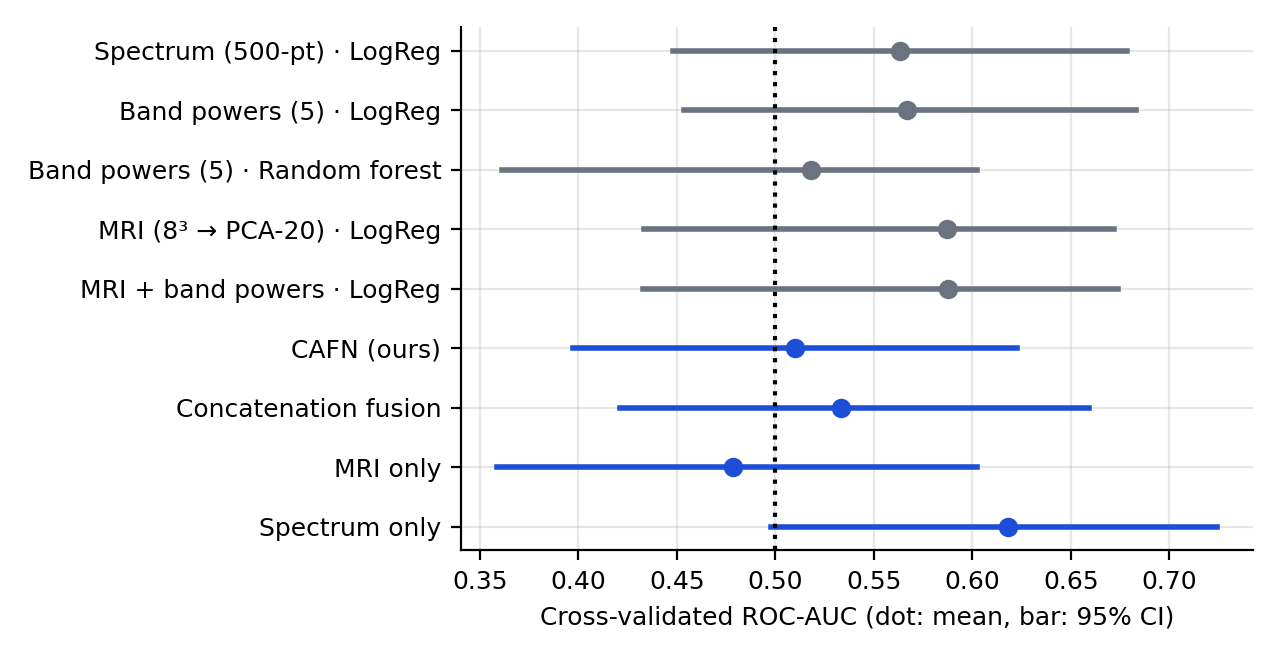
\includegraphics[width=\columnwidth]{results_assets/fig_real_cv.png}
\caption{Cross-validated AUC on the real cohorts (dot: mean, bar: 95\% bootstrap CI). Grey: classical models; blue: neural models. The dotted line is chance.}
\label{fig:realcv}
\end{figure}

\subsection{Cohort split and leave-one-cohort-out}\label{sec:lodo}
Table~\ref{tab:cohortcafn} shows the full CAFN ($64^3$ MRI) trained on the pooled cohorts and evaluated on each cohort's held-out test subjects (7 per cohort), and trained on one cohort and tested on every subject of the other. All accuracies lie between 0.45 and 0.52 and balanced accuracies between 0.46 and 0.54: at chance, with variation across repeats larger than any difference between settings. Fig.~\ref{fig:realcurves} shows why: the training loss falls to nearly zero within 30 epochs while validation accuracy stays near 0.5, i.e.\ the model memorises the roughly 67 training subjects. The classical models do not transfer either (Table~\ref{tab:lodo}): across cohorts the AUC ranges from 0.40 to 0.63 and the balanced accuracy is 0.43--0.51; the spectrum model's AUC of 0.63 when trained on ds007181 and tested on ds003568 comes with a balanced accuracy of 0.50, showing that the ranking transfers weakly while the decision threshold does not (different sensors and recording protocols shift the spectrum). A linear model identifies the cohort from the spectrum alone with 100\% accuracy, so cohort identity is an available shortcut; the within-cohort permutation test in Section~\ref{sec:realcv} is designed not to reward it.

\begin{table}[!t]
\caption{CAFN on the real cohorts (mean $\pm$ SD over 3 repeats; test subjects only).}
\label{tab:cohortcafn}
\centering\scriptsize\setlength{\tabcolsep}{2.5pt}
\begin{tabular}{@{}lccc@{}}
\toprule
Setting & Accuracy & Bal.\ acc. & AUC\\
\midrule
Pooled, test (both cohorts, $n{=}14$) & $0.52\pm0.04$ & $0.52\pm0.04$ & $0.61\pm0.09$ \\
Pooled, test ds003568 ($n{=}7$) & $0.52\pm0.08$ & $0.46\pm0.07$ & $0.61\pm0.17$ \\
Pooled, test ds007181 ($n{=}7$) & $0.52\pm0.08$ & $0.54\pm0.07$ & $0.53\pm0.17$ \\
Leave ds003568 out ($n{=}47$) & $0.48\pm0.09$ & $0.46\pm0.04$ & $0.57\pm0.08$ \\
Leave ds007181 out ($n{=}48$) & $0.45\pm0.02$ & $0.49\pm0.05$ & $0.44\pm0.03$ \\
\bottomrule
\end{tabular}
\end{table}

\begin{table}[!t]
\caption{Leave-one-cohort-out for classical models: AUC / balanced accuracy when tested on the named cohort after training on the other.}
\label{tab:lodo}
\centering\scriptsize\setlength{\tabcolsep}{2.5pt}
\begin{tabular}{@{}lcc@{}}
\toprule
Model & ds003568 & ds007181\\
\midrule
Spectrum (500-pt) $\cdot$ LogReg & 0.63 / 0.50 & 0.57 / 0.50 \\
Band powers (5) $\cdot$ LogReg & 0.50 / 0.50 & 0.48 / 0.50 \\
Band powers (5) $\cdot$ Random forest & 0.50 / 0.50 & 0.50 / 0.50 \\
MRI (8$^3$ $\rightarrow$ PCA-20) $\cdot$ LogReg & 0.40 / 0.43 & 0.44 / 0.47 \\
MRI + band powers $\cdot$ LogReg & 0.41 / 0.43 & 0.46 / 0.51 \\
\bottomrule
\end{tabular}
\end{table}

\begin{figure}[!t]
\centering
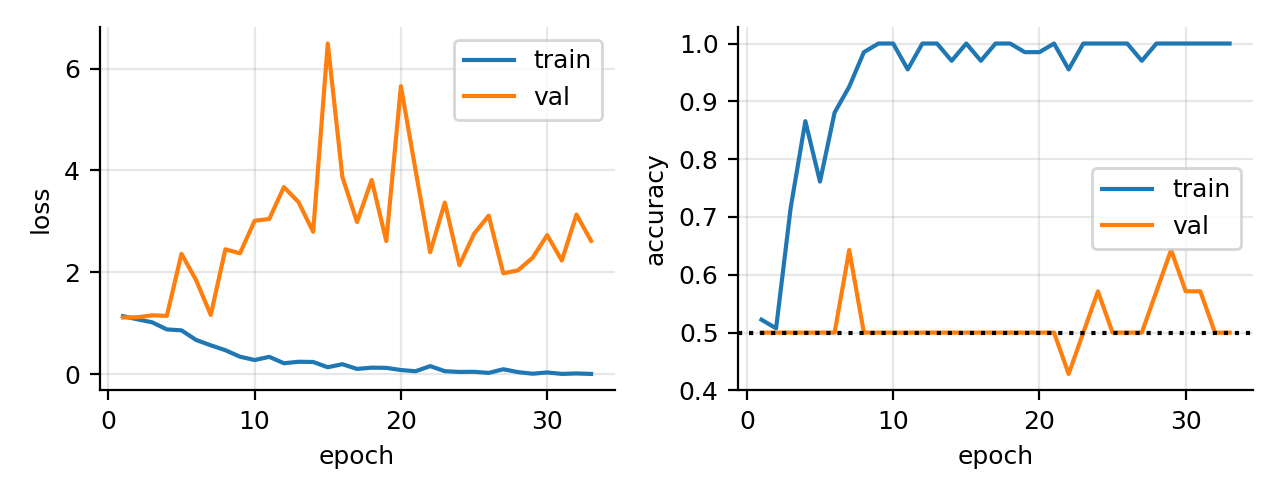
\includegraphics[width=\columnwidth]{results_assets/fig_real_curves.png}
\caption{Pooled CAFN, repeat 0: training versus validation loss and accuracy on the real cohorts. The validation curve stays near chance while the training loss vanishes.}
\label{fig:realcurves}
\end{figure}
